
\lstset{tabsize=2}
\chapter{PDDL}

\section{Blocks domain}\label{blocks}
\subsection{Problem Description}\label{blocks-prob}
\lstinputlisting{appendix/block-problem.pddl}
\subsection{Domain Description}\label{blocks-domain}
\lstinputlisting{appendix/blocks-domain.pddl}


\section{Domain Variation}\label{Domain_Variation}
The original part of the update domain and what its replaced with in the existential approach.
\subsection{Original}\label{domain}
\lstinputlisting{appendix/domain.txt}
\subsection{Changed}\label{domain2}
\lstinputlisting{appendix/domain2.txt}

\chapter{Astro Kid}
\section{Astro Kid Rules}
\label{rules}
An explanation of the basic object and how they behave in the domain. In general these objects obey the law gravity.
\begin{itemize}
	\item{Player} The player can do the following things: walk left and right, climb up and down on ladders, and push objects horizontally away from the player.
	\item{Stone} A movable objects that only moves when pushed.
	\item{Robot} when pushed or activated by a remote moves in straight line forward.
	\item{Teleport} transport only the player two connected teleports.
	\item{gate} A gate blocks it's field until all buttons of the same colour is pressed.
	\item{Ground} four types of ground exists: brown, green (objects stay in motion) purple (poisonous unless wearing boots) and blue (poisonous unless wearing boots).
	\item{Goal} The goal field of the game.
\end{itemize}



\section{Astro Kid Levels}
\begin{figure}
	\centering
	
	\caption{Level 1}
	\label{level1}
	
	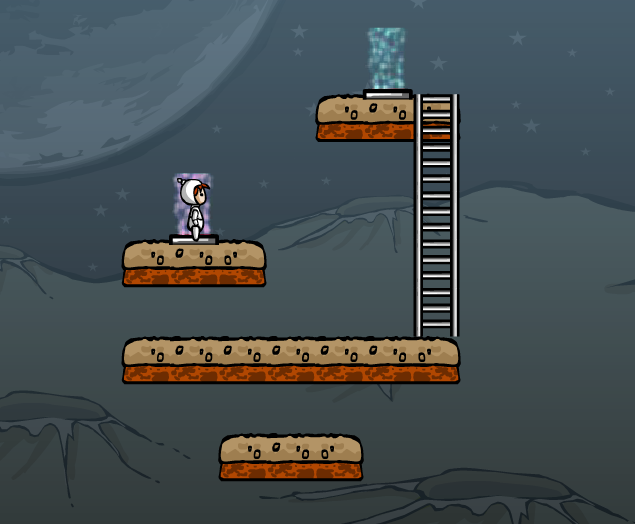
\includegraphics[width=1.0\textwidth]{appendix/img/lvl1}
\end{figure}
\begin{figure}
	\centering
	
	\caption{Level 2}
	\label{level2}
	
	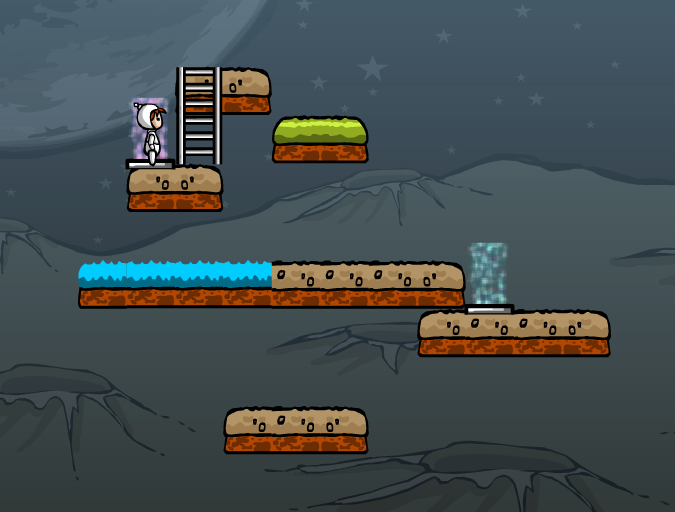
\includegraphics[width=1.0\textwidth]{appendix/img/lvl2}
\end{figure}
\begin{figure}
	\centering
	
	\caption{Level 25}
	\label{level25}
	
	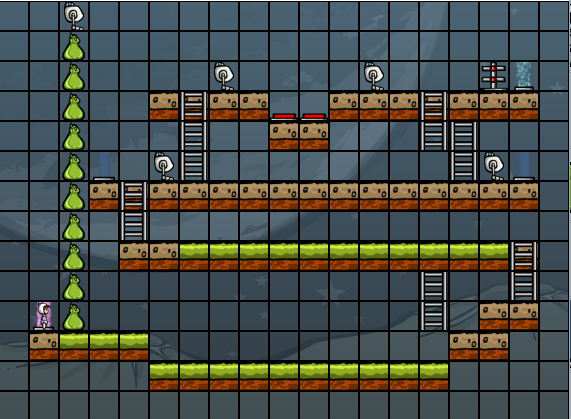
\includegraphics[width=1.0\textwidth]{appendix/img/lvl25}
\end{figure}
\begin{figure}
	\centering
	\caption{Level 31}
	\label{level31}
		
	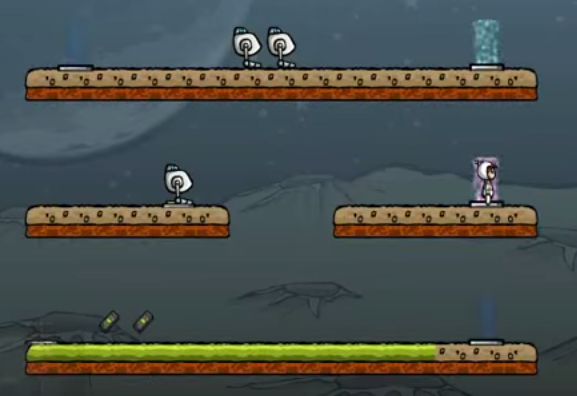
\includegraphics[width=1.0\textwidth]{appendix/img/lvl31}
\end{figure}

\begin{figure}
	\centering
	\caption{Toy problem 1}
	\label{prob01}
	
	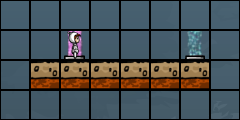
\includegraphics[width=1.0\textwidth]{appendix/img/prob01}
\end{figure}
\begin{figure}
	\centering
	\caption{Toy problem 2}
	\label{prob02}
	
	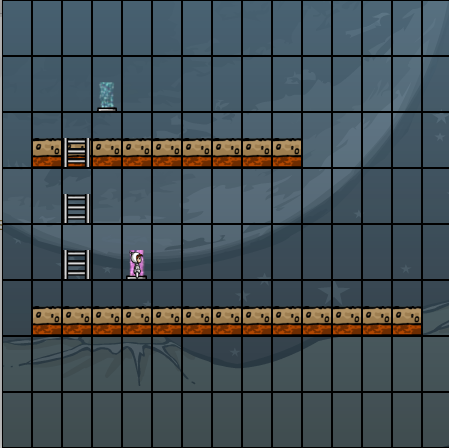
\includegraphics[width=1.0\textwidth]{appendix/img/prob02}
\end{figure}
\begin{figure}
	\centering
	\caption{Toy problem 4v2}
	\label{prob04v2}
	
	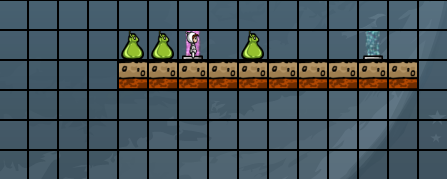
\includegraphics[width=1.0\textwidth]{appendix/img/prob04v2}
\end{figure}
\chapter{Learning}
\section{Grounding}
\label{grounding}
\lstinputlisting{appendix/filtered-action.txt}
\lstinputlisting{appendix/nonfiltered-action.txt}